\subsection{Timing Performance Results for Laser Pulses}
\label{sec:lasertiming}

To characterize the timing performance of the SiPM devices themselves, we
performed laser-based measurements for two types of SiPMs: a Hamamatsu
S12571-015P Multi-Pixel Photon Counter (MPPC) with an area of $1\times
1$~$\mathrm{mm}^{2}$ and pixel pitch size of $15$~$\mu$m, and a Hamamatsu
S12572-25C MPPC with an area of $3\times 3$~$\mathrm{mm}^{2}$ and pixel pitch
size of $15$~$\mu$m. Examples of the digitized waveforms for signals from both
SiPMs are shown in Figure~\ref{fig:pulses}.

\begin{figure}[htbp] 
\centering
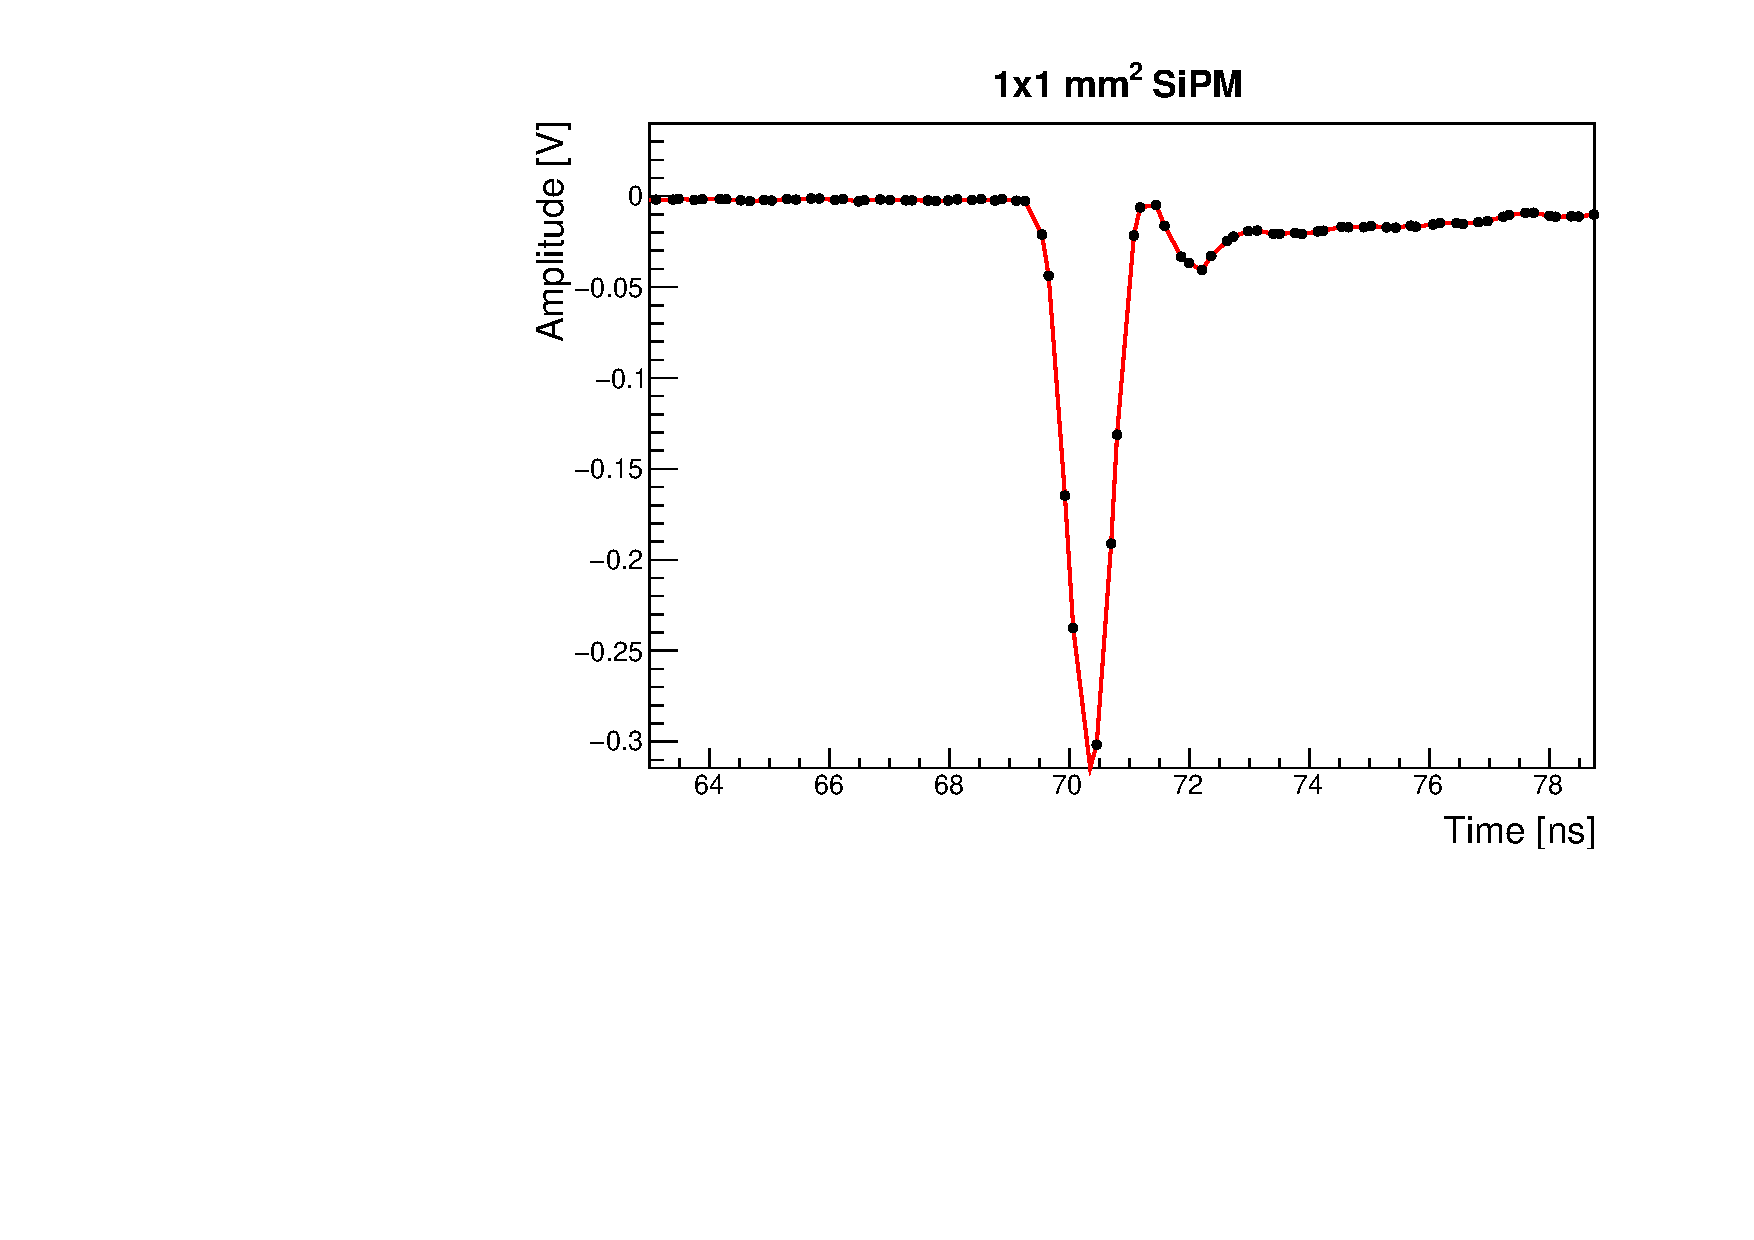
\includegraphics[width=0.49\textwidth]{figures/PulseShapeExample_1x1SiPM.pdf} 
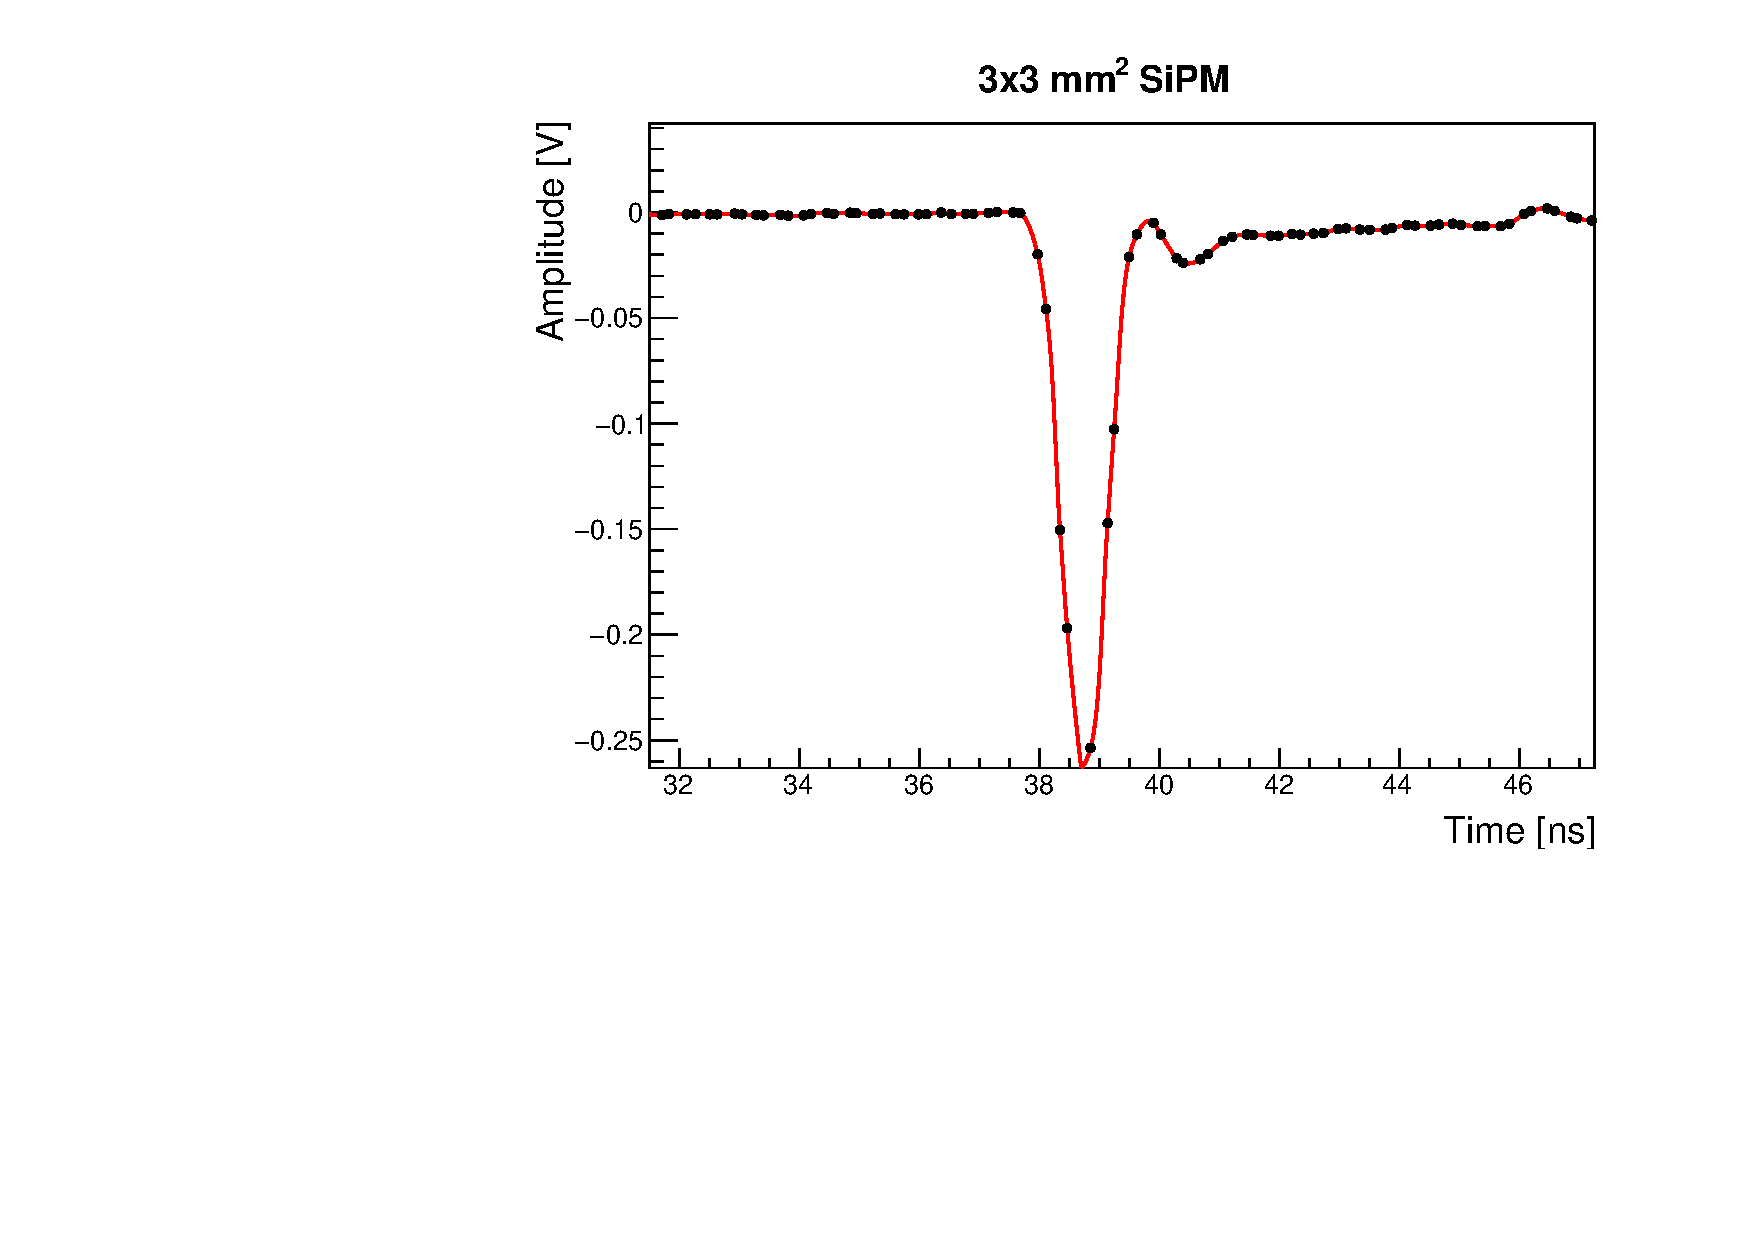
\includegraphics[width=0.49\textwidth]{figures/PulseShapeExample_3x3SiPM.pdf} 
\caption{Digitized waveforms of the signals from the PiLas laser 
in the S12571-015P and S12572-25C SiPMs.} 
\label{fig:pulses} 
\end{figure} 

Using several different ND filters we controlled the intensity of the photon 
beam impinging upon the SiPMs under test and achieved a large dynamic range 
of signal sizes ranging from a single incident photon to a few hundred. In 
Figure~\ref{fig:NPhotonPeaks}, we show the integrated charge distribution
for two example scenarios from which we can clearly distinguish different peaks
corresponding to different number of photoelectrons detected by the SiPMs.

\begin{figure}[htbp] 
\centering
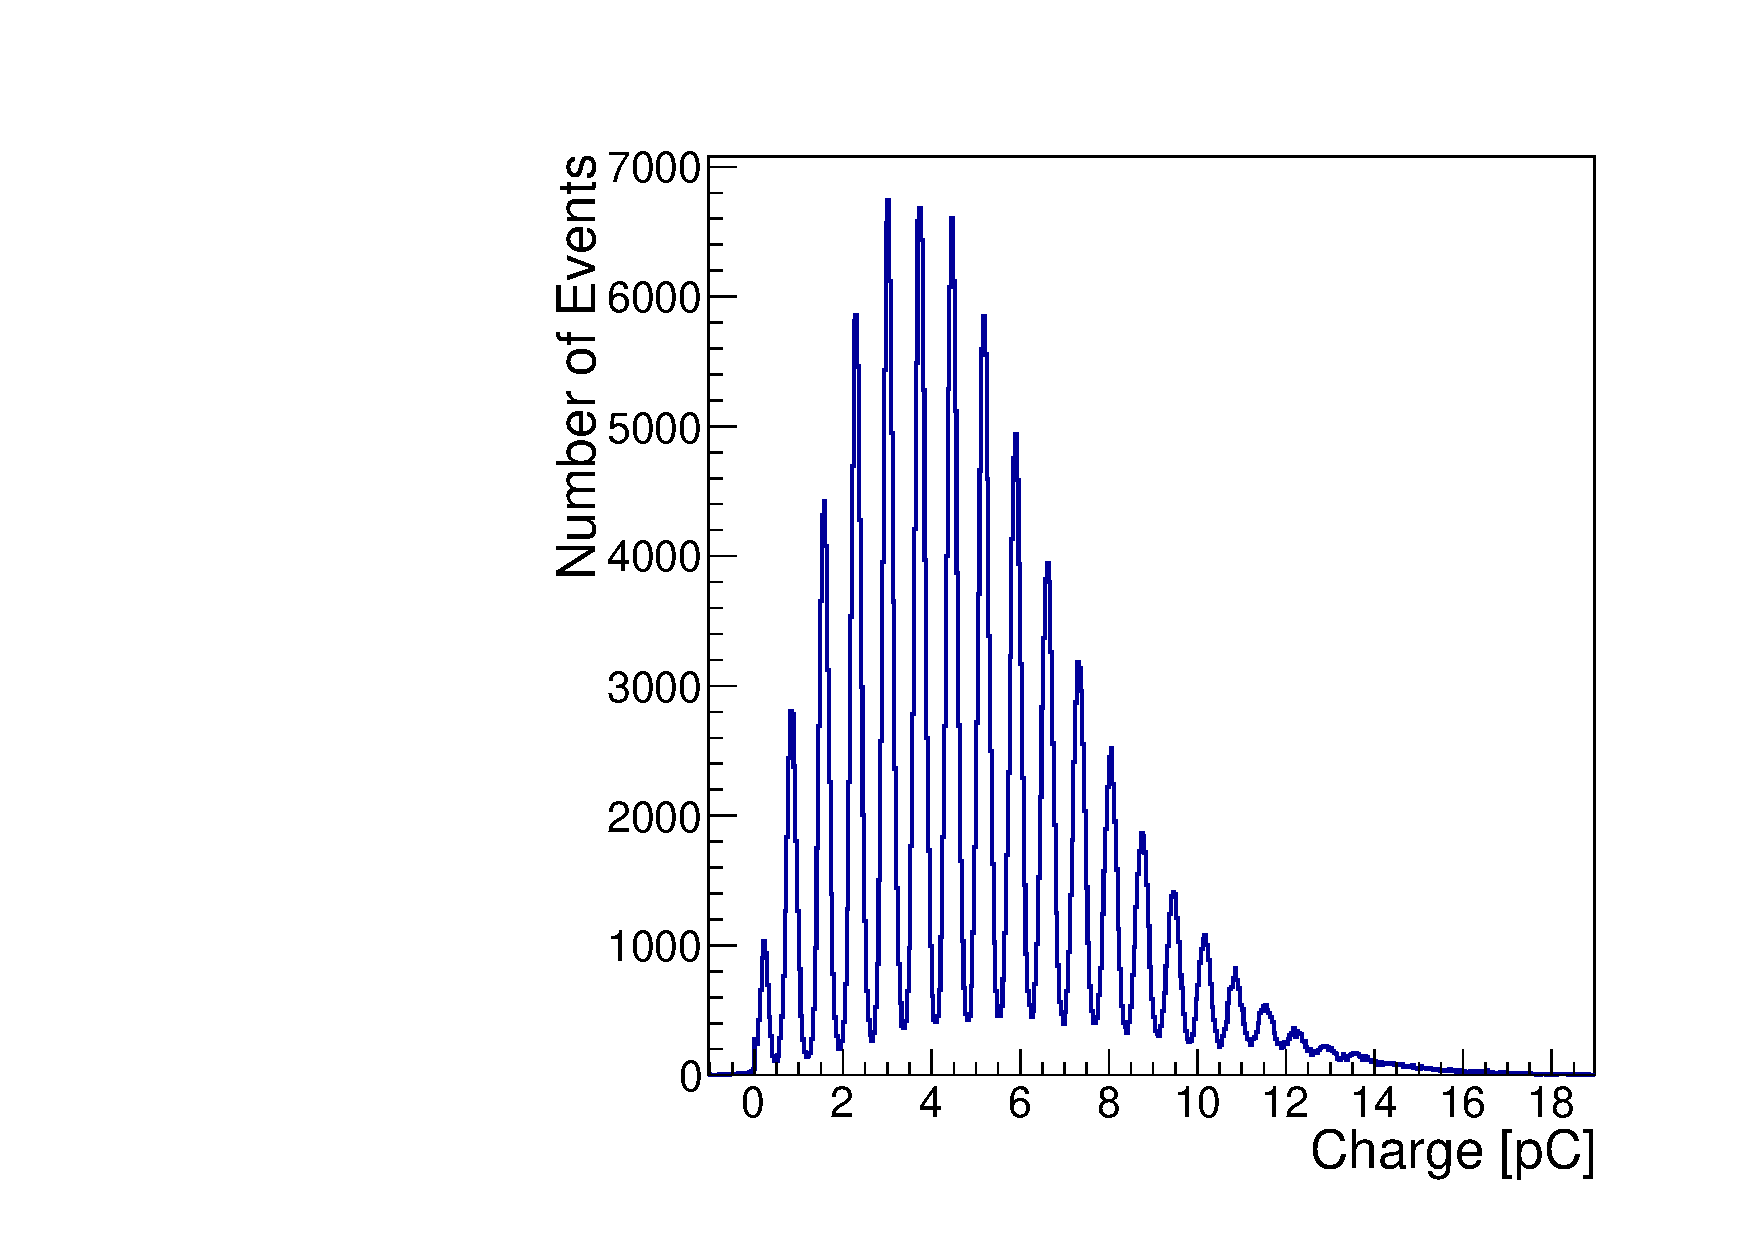
\includegraphics[width=0.49\textwidth]{figures/NPhotons1.pdf} 
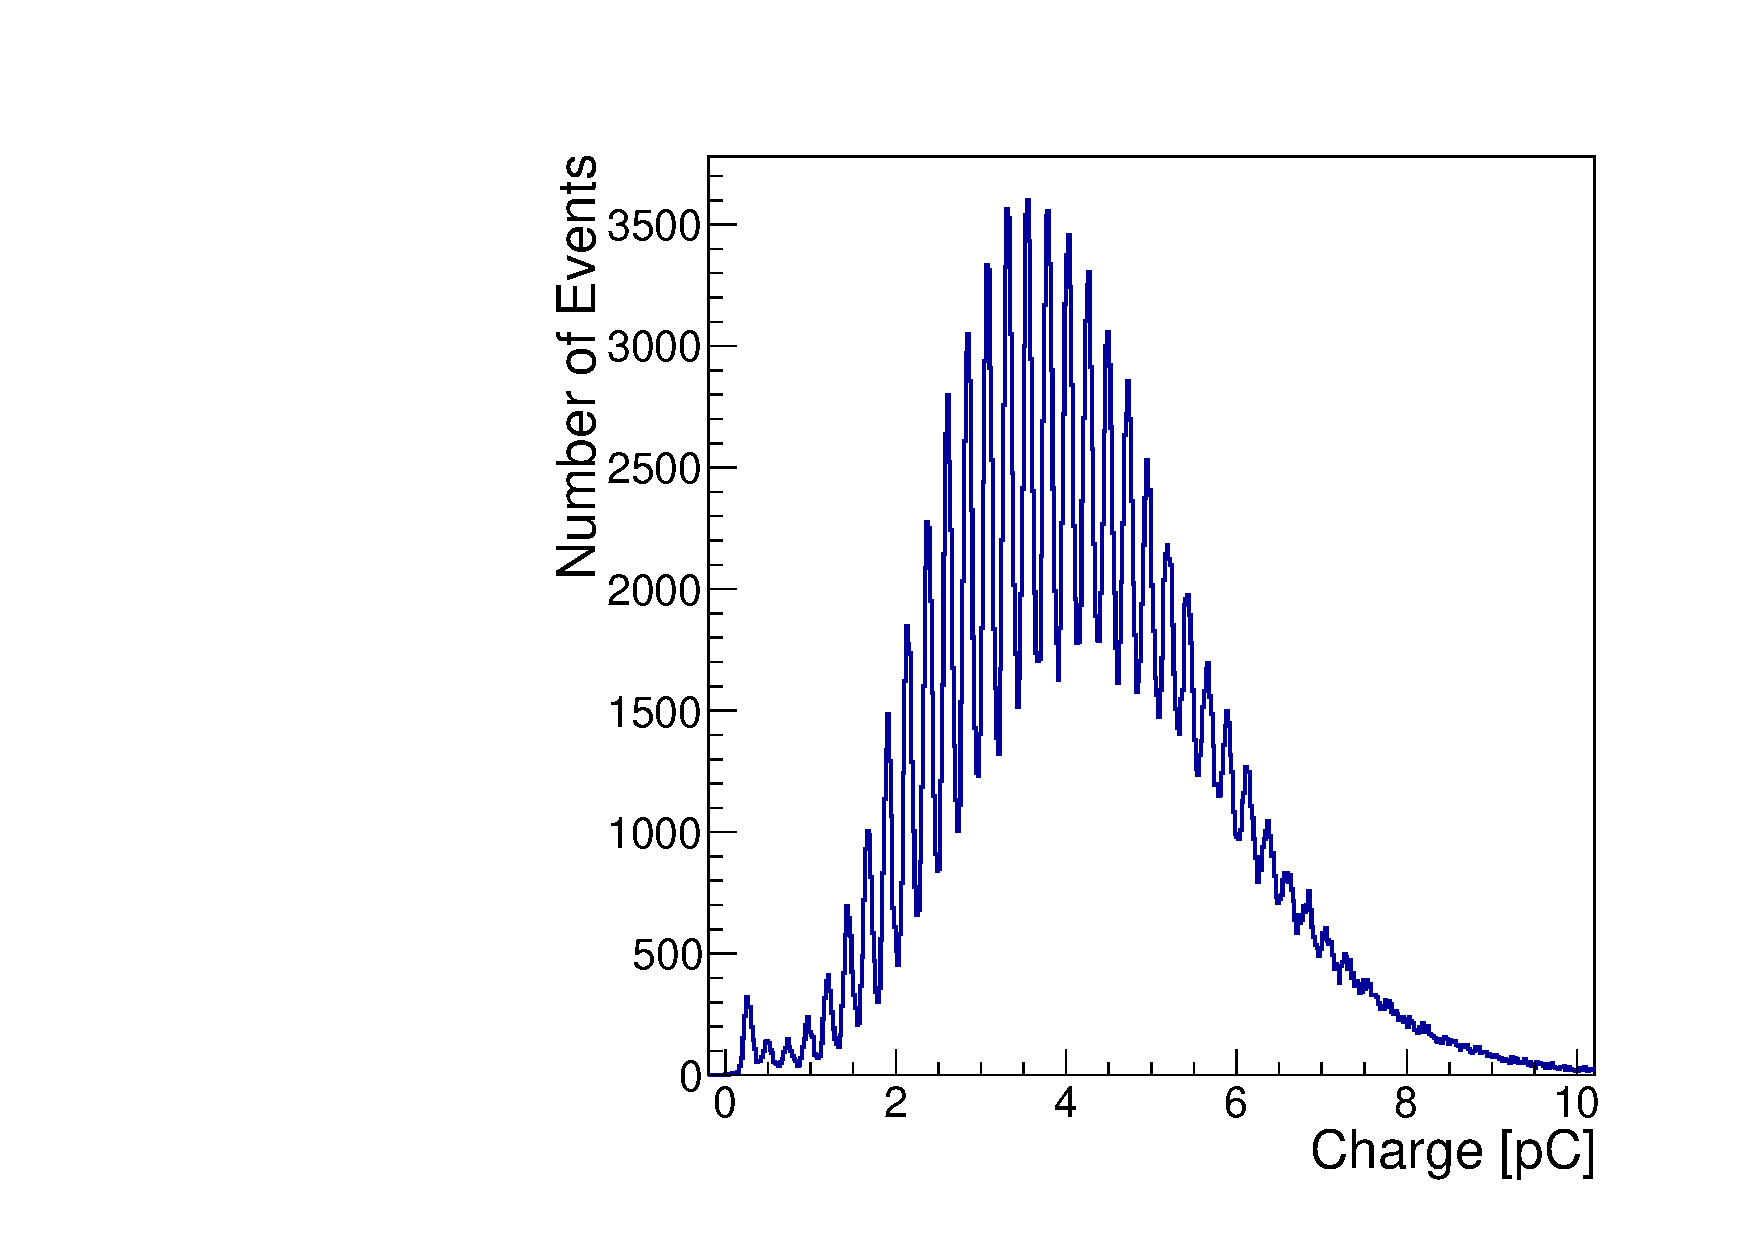
\includegraphics[width=0.49\textwidth]{figures/NPhotons2.pdf} 
\caption{The distribution of integrated charge from the SiPM sensor for data 
taken with an neutral density (ND) filter of 1.8 (left), and an ND filter of 1.4 (right). 
A $10$~db attenuator has been used for the plot on the right. The peaks corresponding
to different discrete numbers of photoelectrons detected by the SiPM is clearly
evident.} 
\label{fig:NPhotonPeaks} 
\end{figure} 

Using this setup, we measure the timestamps reconstructed from the SiPM signals
with respect to the reference MCP-PMT timestamp over an ensemble of events
triggered by the external laser trigger. The sigma parameter of a gaussian fit
to this distribution is taken as the time resolution measurement.
As the number of photons impinging on the SiPM can be clearly distinguished 
based on the amplitude or charge collected, we can study the dependence of the 
time resolution on the number of photons. These measurements are shown in 
Figure~\ref{fig:TimeResolutionVsNPhotons}.


\begin{figure}[htbp] 
\centering
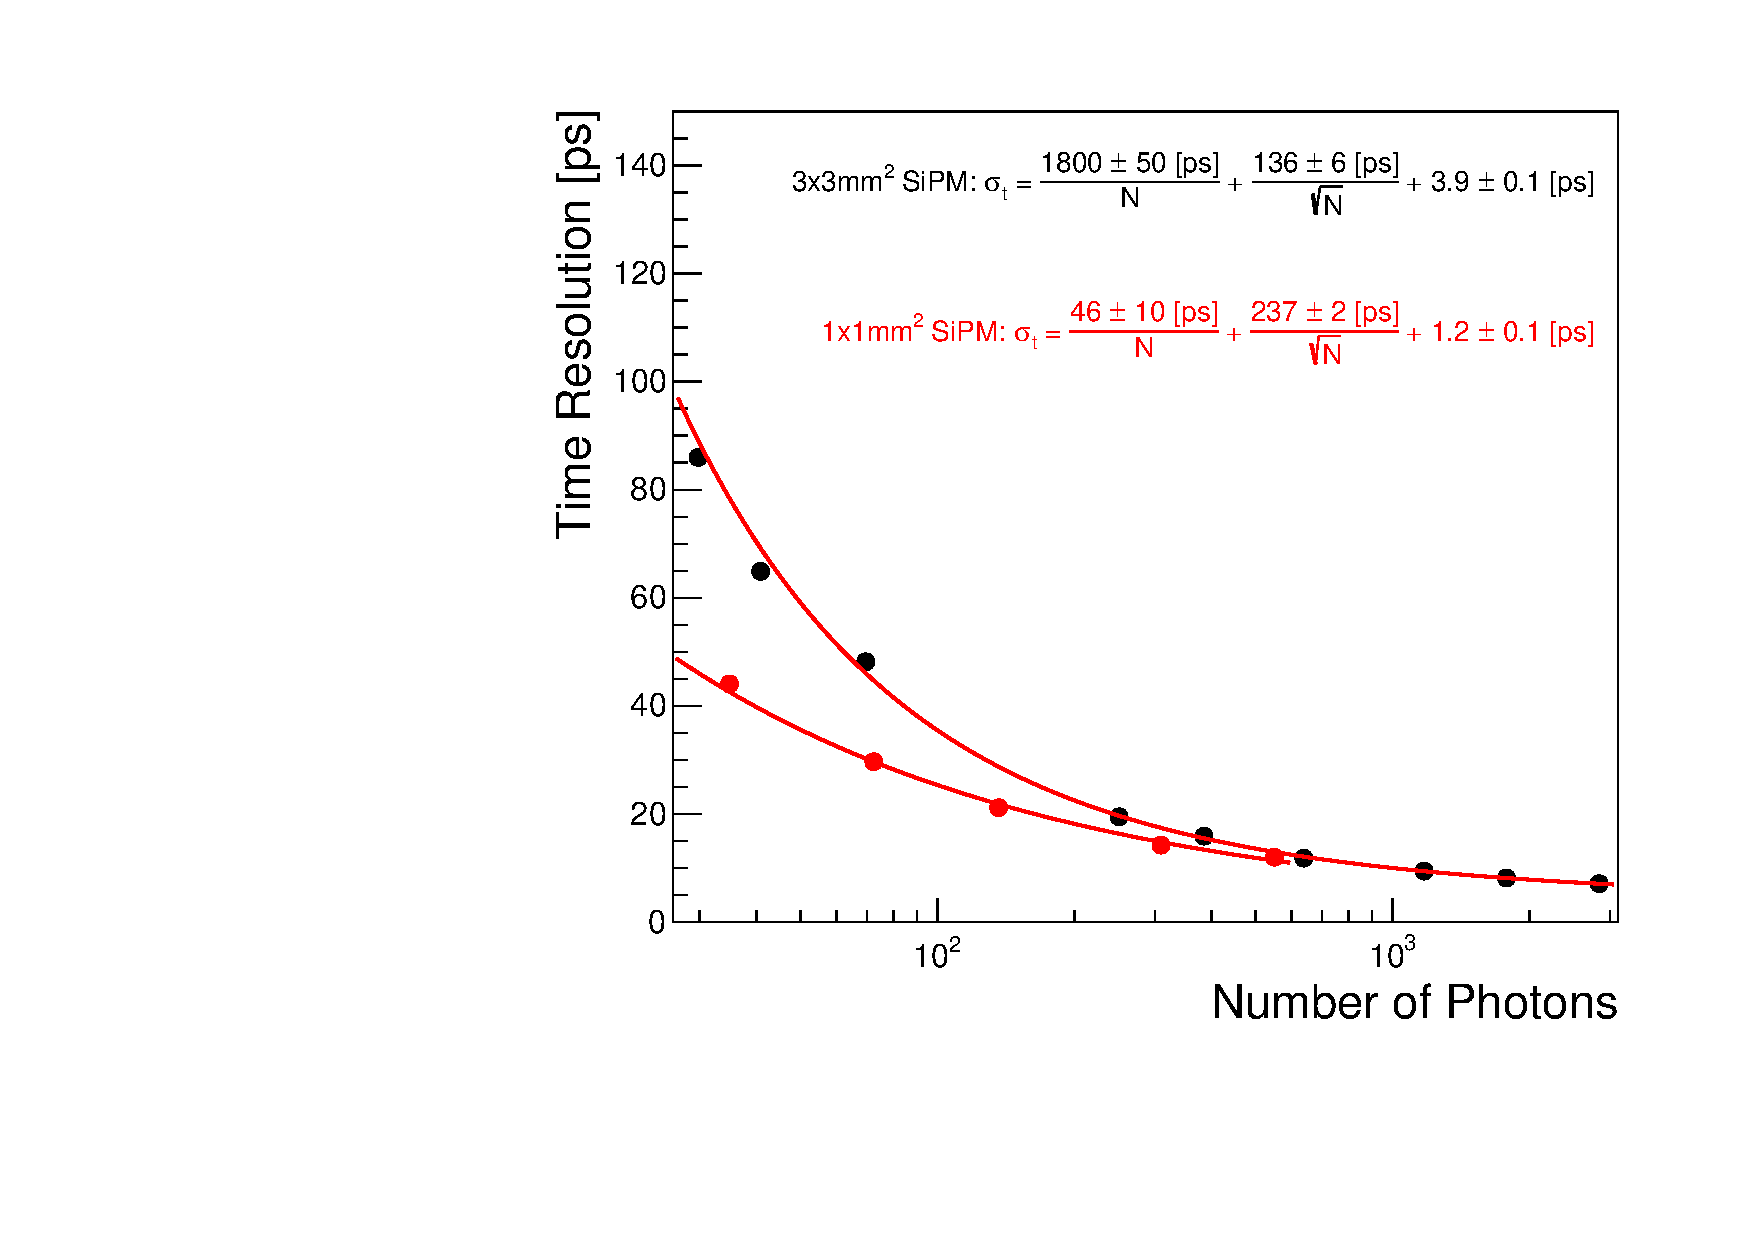
\includegraphics[width=0.49\textwidth]{figures/TimeResolutionVsNPhotons.pdf}
\caption{ The time resolution is measured as a function of the number of photons 
impinging on the SiPMs under test. The black points show measurements using the
$3\times3$~$\mathrm{mm}^{2}$ SiPM, and the red points show measurements
using the $1\times1$~$\mathrm{mm}^{2}$ SiPM. \label{fig:TimeResolutionVsNPhotons}
} 
\label{fig:pulses} 
\end{figure} 


By removing all ND filters and increasing the laser output intensity to near 
maximum, we can measure the time resolution for a very large number of photons 
to probe for the ultimate time resolution that one could achieve with a near 
infinitely large signal. In Figure~\ref{fig:LargeLightTimeResolution} we show 
the SiPM time distributions for such a scenario, and observe that the resolution 
is below the $5$~ps level. The measurement is largely dominated by the limitation
of the digitizer electronics as its impact on the time resolution is $4$~ps. We 
have also performed this measurement using the timestamp associated with the 
external digital trigger signal from the laser and we obtain a result of about 
$11$~ps indicating that the time jitter from the laser trigger signal is roughly 
$10$~ps. 

\begin{figure}[htbp] 
\centering
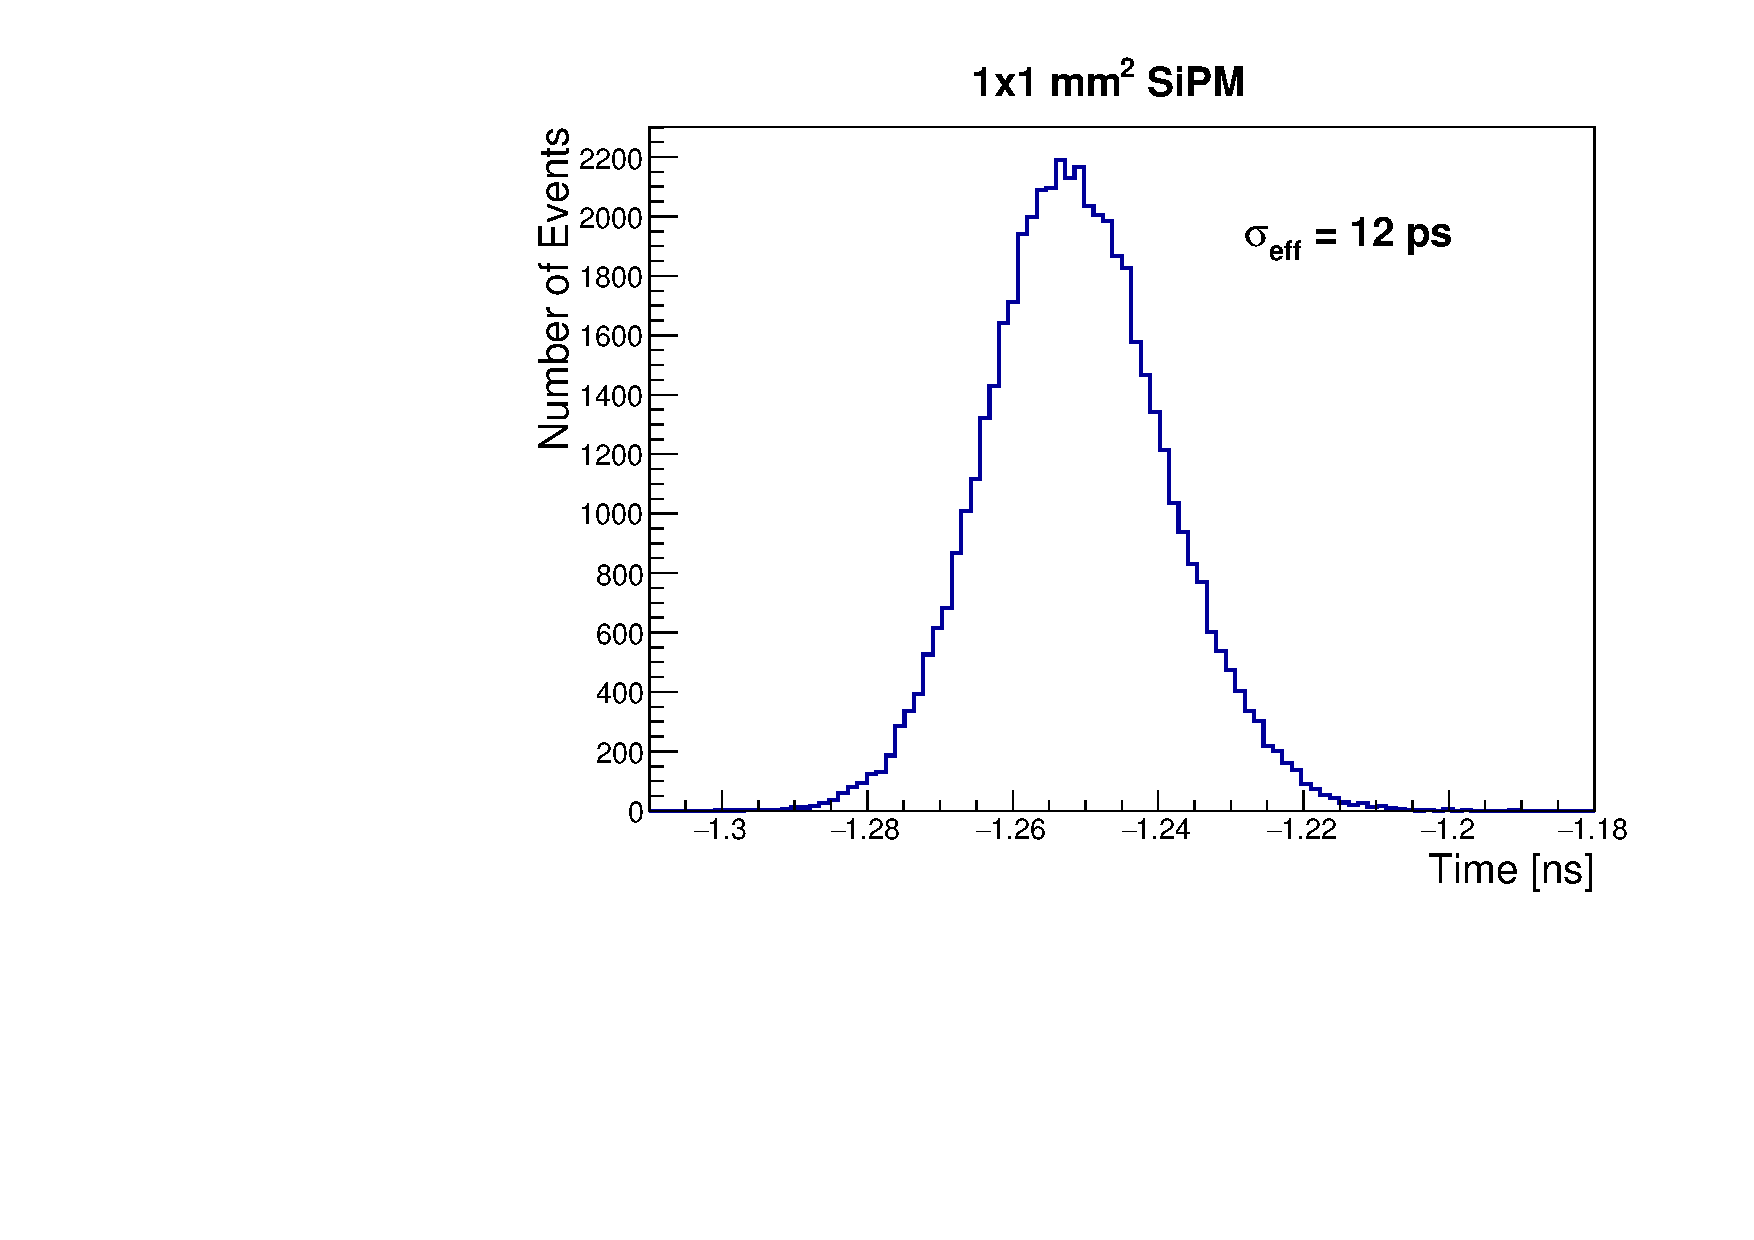
\includegraphics[width=0.49\textwidth]{figures/DeltaT_LargeNPhotons_1x1SiPM.pdf} 
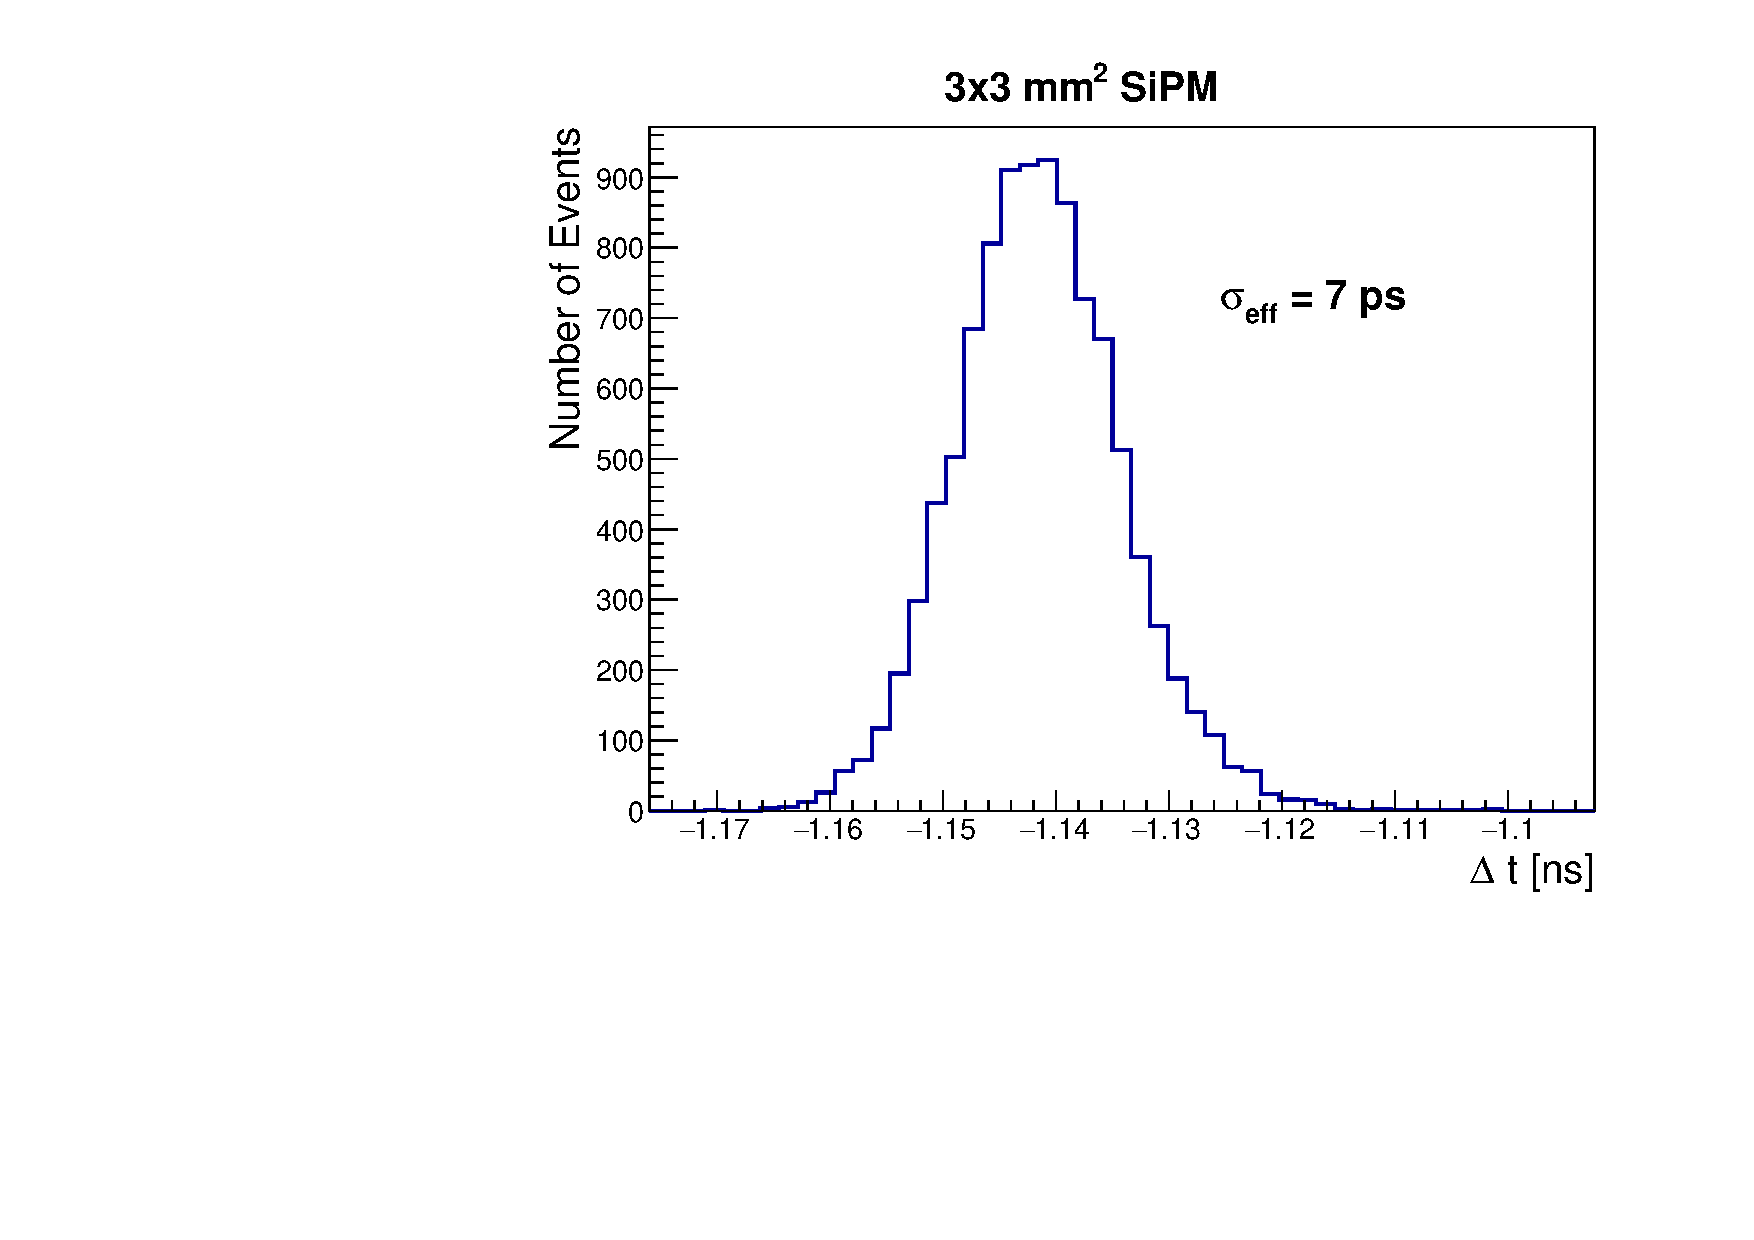
\includegraphics[width=0.49\textwidth]{figures/DeltaT_LargeNPhotons_3x3SiPM.pdf} 
\caption{The SiPM time distribution and resolution measured for laser signals at high laser intensity.} 
\label{fig:LargeLightTimeResolution} 
\end{figure} 

